% !TEX root = ../../../main.tex

\toggletrue{image}
\toggletrue{imagehover}
\chapterimage{genetic_algorithms}
\chapterimagetitle{\uppercase{Genetic Algorithms}}
\chapterimageurl{https://xkcd.com/534/}
\chapterimagehover{Just make sure you don't have it maximize instead of minimize.}

\chapter{Funktionen}
\label{chapter-funktionen}

Wir wollen ein weiteres Mal unsere Programme effizienter gestalten und somit Tipparbeit sparen. Dazu schauen wir uns das Konzept von Funktionen an. Wir können dadurch nicht nur sich wiederholender Quellcode kompakter notieren, sondern unsere Programme auch übersichtlicher und verständlicher gestalten (\say{strukturieren}). Die Lernziele für dieses Kapitel lauten:

\newcommand{\funktionenLernziele}{
\begin{todolist}
\item Sie erklären, was eine Funktion ist und warum der Einsatz einer Funktion hilfreich sein kann.
\item Sie nennen Beispiele von bereits existierenden Funktionen.
\item Sie definieren in Python eine Funktion und rufen Sie an der passenden Stelle auf.
\end{todolist}
}

\lernziel{\autoref{chapter-funktionen}, \nameref{chapter-funktionen}}{\protect\funktionenLernziele}

\funktionenLernziele

\section{Zwei Quadrate \Winkey}

Wir können mit dem Programm aus \autoref{lst-zwei-quadrate} die Figur aus \autoref{figure-zwei-quadrate} zeichnen.

\begin{figure}[htb]
\centering
\begin{minipage}[c][4cm]{0.5\linewidth}
\centering
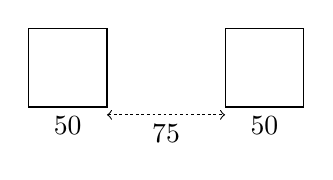
\begin{tikzpicture}
	\draw (0,0) to node [sloped,below] {$50$} ++(1cm, 0) -- ++(0, 1cm) -- ++(-1cm, 0) -- ++(0, -1cm);
	\draw (2.5cm,0) to node [sloped,below] {$50$} ++(1cm, 0) -- ++(0, 1cm) -- ++(-1cm, 0) -- ++(0, -1cm);
	\draw[<->, thin, dashed, dash pattern=on 1pt off 1pt] (1cm,-0.1cm) to node [sloped, below] {$75$} ++(1.5cm, 0);
\end{tikzpicture}
\caption{Zwei Quadrate mit Abstand $75$.}
\label{figure-zwei-quadrate}
\end{minipage}
\hfill
\begin{minipage}[c]{0.4\linewidth}
\centering
\begin{lstlisting}[language=python, caption={Zwei \lstinline{for}-Schleifen nacheinander (\graybgtexttt{zwei\_quadrate.py}).}, label=lst-zwei-quadrate]
import turtle as t

for i in range(4):
    t.fd(50)
    t.lt(90)
t.pu()
t.fd(125)
t.pd()
for i in range(4):
    t.fd(50)
    t.lt(90)
t.done()
\end{lstlisting}
\end{minipage}
\end{figure}

Wir können den Code übersichtlicher gestalten und Tipparbeit sparen, in dem wir eine Funktion definieren und zweimal aufrufen.

\begin{definition}[Funktion]
Mit einer Funktion können wir einen Code-Teil unter einem \textbf{Namen} zusammenfassen und damit an mehreren Stellen \textbf{wiederverwenden}, ohne den Code kopieren zu müssen.
\end{definition}

\autoref{lst-zwei-quadrate-funktion} zeigt den Einsatz einer Funktion am Beispiel der zwei Quadrate. Anstatt den identischen Code zu kopieren, haben wir diesen in eine Funktion gepackt. Dadurch können wir den Code mit einem Funktionsaufruf mehrmals ausführen.

\begin{lstlisting}[language=python, caption={Eine eigene Funktion mit zwei Funktionsaufrufen (\graybgtexttt{zwei\_quadrate.py}).}, label={lst-zwei-quadrate-funktion}]
import turtle


def quadrat_<@\color{black}{50}@>():
    for i in range(4):
        turtle.fd(50)
        turtle.lt(90)


quadrat_<@\color{black}{50}@>()
turtle.pu()
turtle.fd(125)
turtle.pd()
quadrat_<@\color{black}{50}@>()
turtle.done()
\end{lstlisting}

Bisher haben wir \say{nur} bereits bestehende Funktion aufgerufen. Nun definieren wir zuerst eigene Funktionen und rufen diese dann auf. \autoref{figure-funktionen-aufbau} zeigt den Aufbau einer Funktion. Es ist ebenfalls der Zusammenhang von Funktionsdefinition und Funktionsaufruf dargestellt.

\begin{figure}[htb]
\centering
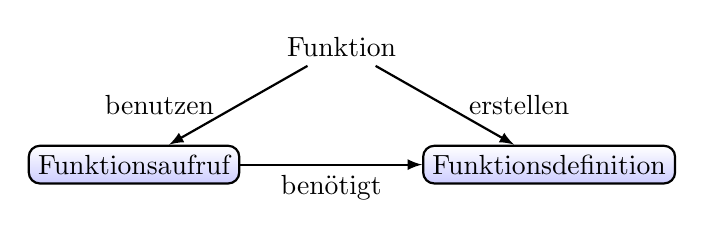
\begin{tikzpicture}[sibling distance=15em, edge from parent/.style = {draw, -latex, thick}]
  \node {Funktion}
    child {	 node[{shape=rectangle, thick, rounded corners,
    draw, align=center, top color=white, bottom color=blue!20}] (call) {Funktionsaufruf} edge from parent node [left, xshift=-0.5em] {benutzen}}
    child { node[{shape=rectangle, thick, rounded corners,
    draw, align=center, top color=white, bottom color=blue!20}] (def) {Funktionsdefinition} edge from parent node [right, xshift=0.5em] {erstellen}};
  \path[-latex, draw, thick] (call) edge node[below] {benötigt} (def);
\end{tikzpicture}
\caption{Aufbau von Funktionen}
\label{figure-funktionen-aufbau}
\end{figure}

\begin{important}[Funktionsdefinition vor Funktionsaufruf]
Prinzipiell gilt: bevor wir eine eigene Funktion aufrufen können, müssen wir die Funktion definieren.
\end{important}

\section{Funktionsdefinition}

Eine Funktionsdefinition besteht aus einem \textbf{Funktionskopf} und einem \textbf{Funktionskörper}. Zuerst wird der Funktionskopf notiert, dann der Funktionskörper.

\subsection{Funktionskopf}

Der Funktionskopf beginnt \textbf{immer} mit dem Schlüsselwort\footnote{Wir haben bereits weitere Schlüsselwörter kennengelernt: \lstinline{import}, \lstinline{for} und \lstinline{in}.} \lstinline{def}. Dies ist eine Abkürzung für \textbf{definition} (dt.: Definition, Festlegung). Das Schlüsselwort \lstinline{def} hat die Bedeutung, dass nun eine Funktionsdefinition beginnt. Mit einem \textbf{zwingenden} Leerzeichen folgt der \textbf{Funktionsname}. Es gelten für den Funktionsnamen dieselben Regeln, wie für Variablennamen. Nach dem Funktionsnamen folgen immer \textbf{runde Klammern}. Eine \mbox{\textbf{öffnende Klammer} \lstinline{(}} und eine \mbox{\textbf{schliessende Klammer} \lstinline{)}}. Die Klammern gehören zur Funktionsdefinition, auch wenn diese momentan noch \say{leer} sind. Danach folgt \textbf{zwingend} ein Doppelpunkt \lstinline{:}.

\subsection{Funktionskörper}

Alle Befehle des Funktionskörpers sind unterhalb des Funktionskopfs in einer neuen Zeile \textbf{eingerückt}. Wie schon bei der \lstinline{for}-Schleife erfolgt die Einrückung (eng. indentation) für alle Befehle des Funktionskörpers einheitlich. Nur die Befehle, die eingerückt sind, gehören zum Funktionskörper und somit zur Funktionsdefinition. Diese Befehle werden beim Funktionsaufruf ausgeführt. Es können \textbf{beliebige Befehle} innerhalb des Funktionskörpers notiert werden.

\begin{example}[Zwei Quadrate]

In \autoref{lst-zwei-quadrate-funktion} ist in Zeile vier der Funktionskopf notiert: \texttt{def quadrat\_50():}. Der Funktionsname lautet \texttt{quadrat\_50}. Der Funktionskörper besteht aus drei Zeilen (Zeile fünf, sechs und sieben). Der Befehl in Zeile zehn (ein Funktionsaufruf) gehört \textbf{nicht} mehr zum Funktionskörper, da der Befehl nicht eingerückt ist.

\end{example}

\begin{cleancode}[Leerzeilen bei der Funktionsdefinition]
\textbf{Vor} und \textbf{nach} einer Funktionsdefinition werden je \textbf{zwei Leerzeilen} eingefügt.
\end{cleancode}

\section{Funktionsaufruf}

Nachdem wir die Funktionsdefinition erläutert haben, schauen wir uns die Ausführung einer Funktion an.

\begin{important}[Funktionsdefinition $\neq$ Funktionsaufruf]
Wenn man eine Funktion definiert, dann werden die Befehle der Funktion noch \textbf{nicht} automatisch ausgeführt.
\end{important}

Wir müssen Python erst \say{sagen}, dass die Funktion ausgeführt werden soll. Mit einem \textbf{Funktionsaufruf} können wir das Ausführen einer Funktion bewirken. Wir sagen Python quasi, führe bitte die Befehle im Funktionskörper jetzt aus. Ein Funktionsaufruf erfolgt durch die Notation des \textbf{Funktionsnamens} und der \textbf{Klammern}. Wir kennen den Funktionsaufruf bereits. Wir haben stets Funktionen aufgerufen, welche \textit{andere} Programmierer erstellt haben. Beispiele:

\begin{itemize}
\item \lstinline{forward(100)}
\item \lstinline{print("Hello, World!")}
\item \lstinline{input("Zahl? ")}
\item \lstinline{sqrt(42)}
\end{itemize}

Neu ist nun, dass wir auch noch unsere eigenen Funktionen aufrufen.

\begin{hinweis}
Der Funktionsaufruf von eigenen Funktionen unterscheidet sich nicht vom bisherigen Funktionsaufruf. Wir verwenden \textbf{nicht} \lstinline{def} beim Funktionsaufruf oder den Doppelpunkt. Einziger Unterschied: Unsere Funktionsdefinitionen besitzen noch keine Parameter für den Funktionsaufruf mit einem Argument. Aber auch dies können wir noch einfügen.
\end{hinweis}

Wir können eine Funktion beliebig oft aufrufen. Egal, wann wir eine Funktion aufrufen, es werden immer die Befehle innerhalb des Funktionskörpers exakt einmal pro Funktionsaufruf ausgeführt.

\begin{important}
Befindet sich die Funktionsdefinition in der gleichen Python-Datei wie der Funktionsaufruf, dann ist keine \lstinline{import}-Anweisung notwendig. Wir können die Funktion direkt aufrufen. Andernfalls ist die übliche Notation mit dem \say{Punkt} zu verwenden.
\end{important}

\begin{example}[Zwei Quadrate]

In \autoref{lst-zwei-quadrate-funktion} rufen wir zweimal unsere eigene Funktion auf. In Zeile zehn und 14: \texttt{quadrat\_50()}.

\end{example}

\section{Wie wählen wir Funktionsnamen?}

Innerhalb der üblichen Regeln sind wir grundsätzlich frei bei der Wahl des Funktionsnamens. Jedoch sollte man einen Funktionsnamen so wählen, dass man allein durch den Funktionsnamen weiss, was die Befehle im Funktionskörper bewirken.

\begin{cleancode}[Sinnvolle Funktionsnamen]
Wir wählen \textbf{Funktionsnamen} so, dass wir direkt verstehen was die Funktion macht. Wir verwenden keine Grossbuchstaben und trennen einzelne Wörter durch einen Unterstrich (\lstinline{_}).
\end{cleancode}

\begin{example}[Zwei Quadrate]

Der Funktionsname \texttt{quadrat\_50} aus \autoref{lst-zwei-quadrate-funktion} deutet direkt darauf hin, was die Funktion macht: Es wird ein Quadrat mit der Seitenlänge $50$ gezeichnet.

\end{example}

\section{Aufgaben}

In den folgenden Aufgaben setzen Sie sich mit dem Erstellen von eigenen Funktionen auseinander.

\subsection{Aufgabe 1}

Notieren Sie ein Programm, welches mit der Turtle die beiden \textbf{gleichseitigen Dreiecke} aus \autoref{figure-zwei-dreiecke} zeichnet. Erstellen Sie eine Funktionsdefinition \lstinline{def dreieck_100():} und notieren Sie darin die Funktionsaufrufe zum Zeichnen \textbf{eines} Dreiecks. Verwenden Sie im \textbf{Funktionskörper} eine \lstinline{for}-Schleife. Rufen Sie die Funktion dann \textbf{zweimal} auf, um die ganze Figur zu zeichnen.

\begin{figure}[htb]
\centering
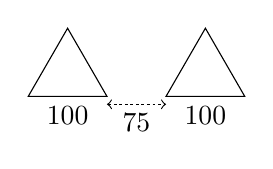
\begin{tikzpicture}
	\draw (0,0) to node [sloped, below] {$100$} ++(1cm, 0) -- ++(-0.5cm, 0.866cm) --cycle;
	\draw (1.75,0) to node [sloped, below] {$100$} ++(1cm, 0) -- ++(-0.5cm, 0.866cm) --cycle;
	\draw[<->, thin, dash pattern=on 1pt off 1pt] (1cm,-0.1cm) to node [sloped, below] {$75$} ++(0.75cm, 0);
\end{tikzpicture}
\caption{Zwei gleichseitige Dreiecke.}
\label{figure-zwei-dreiecke}
\end{figure}

\fillwithgrid{3.5in}

\subsection{Aufgabe 2}

Notieren Sie ein Programm, welches mit der Turtle die \textbf{sechs Quadrate} aus \autoref{figure-quadrate-funktionen} zeichnet. Erstellen Sie eine Funktionsdefinition mit dem Namen \lstinline{quadrat_100} und notieren Sie im Funktionskörper die Funktionsaufrufe zum Zeichnen \textbf{eines} Quadrats (\lstinline{for}-Schleife verwenden). Rufen Sie die Funktion dann mit einer \lstinline{for}-Schleife \textbf{sechsmal} auf, um die ganze Figur zu zeichnen.

\begin{figure}[htb]
\centering
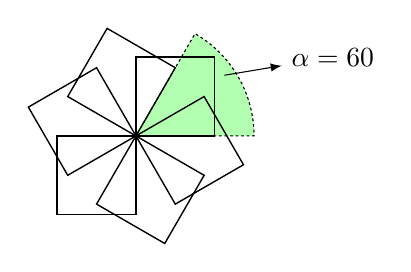
\begin{tikzpicture}
	\draw[fill=green!30, thin, dash pattern=on 1pt off 1pt] (0,0) -- ++(0:1.5cm) arc (0:60:1.5cm) -- (0,0);
	\draw[line width=0.5pt] (0,0) rectangle (1,1);
	\draw[line width=0.5pt, rotate around={60:(0,0)} ] (0,0) rectangle (1,1);
	\draw[line width=0.5pt, rotate around={120:(0,0)} ] (0,0) rectangle (1,1);
	\draw[line width=0.5pt, rotate around={180:(0,0)} ] (0,0) rectangle (1,1);
	\draw[line width=0.5pt, rotate around={240:(0,0)} ] (0,0) rectangle (1,1);
	\draw[line width=0.5pt, rotate around={300:(0,0)} ] (0,0) rectangle (1,1);
	\node (A) at (1,0.75) {};
	\node (B) at (2.5, 1) {$\alpha = \qty{60}{\degree}$};
	\draw[-latex] (A) -- (B);
\end{tikzpicture}
\caption{Nach jedem Quadrat dreht sich die Turtle um $\qty{60}{\degree}$ nach links.}
\label{figure-quadrate-funktionen}
\end{figure}

\vspace{-0.75cm}

\fillwithgrid{3in}

\section{Funktionen kombinieren}

Natürlich können wir auch mehrere Funktionen definieren und die Funktionsaufrufe miteinander kombinieren. \autoref{lst-zwei-quadrate-zwei-funktion} zeigt nochmals das Eingangsbeispiel mit zwei Funktionsdefinitionen.

\begin{lstlisting}[language=python, caption={Zwei Funktionsdefinitionen. In der zweiten Funktionsdefinition wird die erste Funktion durch die Schleife mehrfach aufgerufen.}, label={lst-zwei-quadrate-zwei-funktion}]
import turtle


def quadrat_<@\color{black}{50}@>():
    for i in range(4):
        turtle.fd(50)
        turtle.lt(90)


def quadrate():
    for j in range(2):
        quadrat_<@\color{black}{50}@>()
        t.pu()
        t.fd(125)
        t.pd()


quadrate()
t.done()
\end{lstlisting}